%!TEX root = ../thesis.tex

% Definitions:
%%%%%%%%%%%%%%
% Semantiv Web = samantisches Web

\chapter{Grundlagen} % (fold)
\label{cha:grundlagen}

\section{Datenintegration} % (fold)
\label{sec:datenintegration}

% section datenintegration (end)


\subsection{Semantic web und das Resource Description Framework} % (fold)
\label{sub:semantic_web_und_das_resource_description_framework}



\todo[inline]{Idee semantic web einbauen}
\todo[inline]{Use cases, Vision und Anforderungen. Auf die kann dann in der Analyse genauer drauf eingegangen werden}

Eine der bekanntesten Umsetzungen der Vision des  semantischen Webs ist wohl das Resource Description Framework (RDF). Wie der Name schon suggeriert dient RDF zur Beschreibung von einzelnen Ressourcen innerhalb des Internets. Nach \cite{Klyne2004,Manola2004} bestand die Motivation bei der Entwicklung von RDF Information über Ressource in einen offenen Datenmodell zu speichern, so dass diese Daten von Maschinen automatisch verarbeitet, manipulieren und untereinander ausgetauscht werden können. Gleichzeitig sollte es auch einfach von jedem erweitert werden können \enquote{RDF is designed to represent information in a minimally constraining, flexible way}\cite{Klyne2004}.

\medskip

Das Datenmodell von RDF ist sehr einfach aufgebaut um es effizient verarbeiten zu können. Die Grundlage bilden simple Tripel aus Subjekt, Prädikat und Objekt, welche an die natürliche Sprache angelehnt als Sätze\cite{Heinzen} bezeichnet werden. Mehrere solcher Tripel bilden einen RDF Graphen. Das Prädikat beschreibt hierbei eine Beziehung zwischen Subjekt und Objekt und wird daher oft als Eigenschaft beschrieben. In der natürlichen Sprache kann man dies zum Beispiel so ausdrücken; Das Subjekt hat eine Eigenschaft mit den Wert Objekt. Graphisch wird dies durch eine gerichtete Verbindung von Subjekt und Objekt mit der Beschriftung der Prädikats dargestellt (siehe Abbildung \ref{fig:graphische_darstellung_eines_rdf_tripels}).

\medskip

\begin{figure}[h]
    \centering
    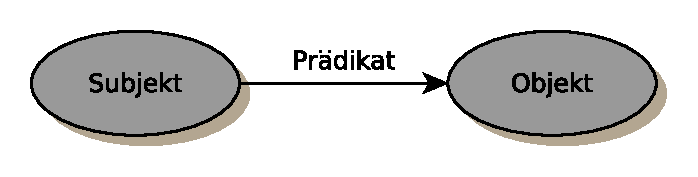
\includegraphics[scale=0.7]{assets/images/rdf-triple}
    \caption{Graphische Darstellung eines RDF Tripels}
    \label{fig:graphische_darstellung_eines_rdf_tripels}
\end{figure} 

Für Subjekt, Prädikat und Objekt besteht die Möglichkeit sogenannte Uniform Resource Identifiers (URI), Literale oder leere Knoten als Werte einzusetzen. 

\begin{description}
    \item[URIs] sind eindeutige Bezeichner die eine beliebige reale oder abstrakte Ressource und werden wie in RFC 2396\footnote{\url{http://www.isi.edu/in-notes/rfc2396.txt}} beschrieben formatiert, wobei relative URIs nach \cite{Klyne2004} nicht verwendete werden sollen.
    \item[Literale] bestehen aus einfachen Zeichenketten die zum Speichern der Informationen dienen. Zusätzlich können Literale mit der Angabe der verwendeten Sprache \lstinline[basicstyle=\ttfamily]{"Objekt"@de} oder des Datentyps \lstinline[basicstyle=\ttfamily]{"42"^^xsd:integer} erweitert werden. Bei Literalen ist aber auch darauf zu achten, dass \lstinline[basicstyle=\ttfamily]{"Objekt} und \lstinline[basicstyle=\ttfamily]{"Objekt"@de} beschreiben zwar beide den gleichen Wert werden aber von RDF nicht als gleich angesehen. Zwei Literale können nur gleich sein, wenn sie die selbe Sprache beziehungsweise den selben Datentyp besitzen.  
    \item[Leere Knoten] werden als alle Knoten im RDF Graphen beschrieben, welche weder eine URI noch ein Literal sind. Sie dienen häufig dazu um Subjekte zu beschreiben für die aber nicht unbedingt eine eigene URI nötig ist und sind nur innerhalb eines Graphen eindeutig\todo{Daher eignen sie sich auch nicht zur Referenzierung außerhalb des RDF-Graphen!} \todo[inline]{Beispiel}.
\end{description}

Doch nicht jeder davon ist in jeden Teil des Tripels erlaubt. Das Subjekt ist entweder eine URI oder ein leerer Knoten wobei das Prädikat nur eine URI sein kann. Dahingegen ist es beim Objekt möglich eine URI, einen leeren Knoten oder ein Literal zu verwendeten. 

\subsubsection{RDF Darstellungsformate} % (fold)
\label{ssub:rdf_xml_n3}

\begin{description}
    \item[RDF/XML] 
    \item[N3] ist die Kurzform für Notation 3 und wurde von Tim Berners-Lee als Sprache für RDF entwickelt. Tripel in N3 werden dabei wie Sätze in meisten natürlichen Sprachen geschrieben. Erst das Subjekt, dann das Prädikat und am Ende das Objekt gefolgt von einen Punkt, wie in  Listing \ref{lst:n3_beispiel} zu sehen ist.
    \begin{lstlisting}[caption={Einfaches N3 Beispiel}\label{lst:n3_beispiel},captionpos=t]
<http://example.de/florian> <http://example.org/#name> "Florian" .
<http://example.de/florian> <http://example.org/#age> "28" .    \end{lstlisting} 
    Die URI \texttt{http://example.de/florian} beschreibt hierbei eine Ressource welche einen Namen \texttt{Florian} und ein Alter \texttt{28} besitzt. Es ist darauf zu achten, dass alle URI immer zwischen spitzen Klammern stehen. Da nun einzelne Prädikate recht häufig innerhalb eines Graphen auftauchen können, kann es einfach sein diese abgekürzt schreiben zu können. Hierzu ist es möglich sogenannte Präfixe (auch Namensräume genannt) am Beginn des Dokumentes zu definieren und einen so Schreibarbeit abzunehmen.

    \begin{lstlisting}[caption={Präfixe}\label{lst:n3_prefix},captionpos=t]
@prefix person: <http://example.org/#> .
<http://example.de/florian> person:name "Florian" .
<http://example.de/florian> person:age "28" .    \end{lstlisting}

    Am Anfang von Listing \ref{lst:n3_prefix} wird durch Einleiten mittels des Schlüsselwortes \texttt{@prefix} ein neuer Präfix \texttt{person:} für die URI \texttt{http://example.org/\#} festgelegt (man beachte wieder den Punkt am Ende der Zeile). Dieser Präfix kann nun überall innerhalb des Dokumentes verwendet werden, wobei die spitzen Klammern der vorherigen URI weggelassen werden können.

    \todo[inline]{Leere Knoten + kurz Turtle}
    \todo[inline]{Die englischen Fachbegriffe (also hier blank nodes oder bnodes) würde ich auch erwähnen. Das hilft dem Leser, wenn er sich englischsprachige Literatur anschaut nach dem er deine Arbeit gelesen hat.}

\end{description}

% subsubsection rdf_xml_n3_turtle (end)

\subsubsection{Abfragesprache SPARQL} % (fold)
\label{ssub:abfragesprache_sparql}

% subsubsection resource_description_language (end)

\subsubsection{Ontologien} % (fold)
\label{ssub:ontologien}

% subsubsection ontologien (end)

% subsection semantic_web_und_das_resource_description_framework (end)

\section{Semantically-Interlinked Online Communities} % (fold)
\label{sec:verw_arbeiten_sioc}

Semantically-Interlinked Online Communities\footnote{\url{http://sioc-project.org/}} (SIOC, ausgesprochen \enquote{schock}) ist ein Projekt, welches von Uldis Boj\=ars und John Breslin begonnen wurde um unterschiedliche, webbasierte Diskussionslattformen(Blog, Forum, Mailinglist,\dots) untereinander verbinden zu können \cite{Breslin2005}. Der Kern von SIOC besteht aus einer Ontologie, welche den Inhalt und die Struktur diese Plattformen in ein maschinenlesbares Format bringt und es erlaubt diese auf semantischer Ebene zu verbinden. Auch soll es so möglich sein Daten von einer Plattform zu einer Anderen zu transferieren und so einfacher Inhalte austauschen zu können. Als Basis für SIOC dient RDF, die Ontologie selber wurde in RDFS und OWL designt. Um nicht das Rad neu erfinden zu müssen greift SIOC auf schon bestehende und bewährte Ontologien zurück. Für die Abbildung von Beziehungen zwischen einzelnen Personen wird Friend of a Friend\footnote{\url{http://www.foaf-project.org/}} (FOAF) und für einige Inhaltliche- und Metadaten (Titel, Inhalt, Erstelldatum, \dots) Dublin Core Terms\footnote{http://dublincore.org/documents/dcmi-terms/} eingesetzt.

\begin{figure}[ht]
    \centering
    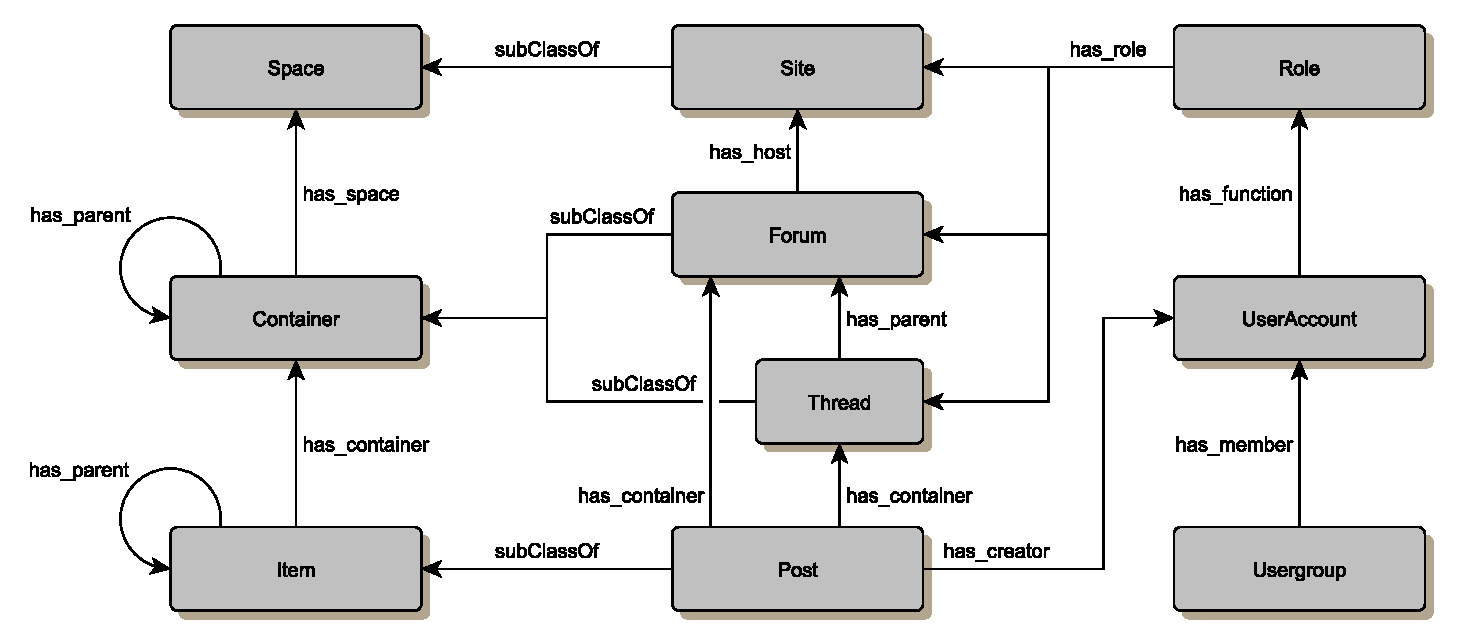
\includegraphics[
        width=\textwidth,
        keepaspectratio=true,
        clip=true]
        {assets/images/sioc_overview}
    \caption{Aufbau von SIOC (modifiziert) - Originalquelle: \cite{deri2013}}
    \label{fig:sioc_aufbau_diagramm}
\end{figure}

\section{Datenverteilung} % (fold)
\label{sec:datenverteilung}

\subsection{Enterprise Integration Pattern} % (fold)
\label{sub:enterprise_integration_pattern}

% subsection enterprise_integration_pattern (end)

\subsection{Java Messaging Service} % (fold)
\label{sub:java_messaging_service}

% subsection java_messaging_service (end)

\subsection{Apache Camel} % (fold)
\label{sub:apache_camel}

% subsection apache_camel (end)

% section datenverteilung (end)

\todo[inline]{Du könntest in dem Grundlagenkapitel auch noch auf Foren, Moodle, FB und Google+ kurz eingehen. Deren Datenmodelle und -schnittstellen können auch später erläutert werden.}


\section{Verwandte Arbeiten und Projekte} % (fold)
\label{sec:verwandte_arbeiten_und_projekte}

\subsection{Reclaim Social} % (fold)
\label{sub:verw_arbeiten_reclaim_social}

Hat sich nicht jeder schon einmal vor den Rechner gesessen um, zum Beispiel, nach einen Bild gesucht das man irgendwann auf irgendeinem der unzähligen sozialen Netzwerke hochgeladen hat, einem aber partout nicht einfallen will wo? Wann und wo habe habe ich den Beitrag geschrieben, der perfekt zu meiner aktuellen Arbeit passen würde? Solche oder ähnliche Fragen wurden sicherlich schon mehrere Millionen mal von verschiedenen Menschen in der Welt des Internets gestellt. Wer hätte in so einen Fall nicht gerne alles was man über die letzten Jahre an verschiedenen Stellen im Netz geschrieben, hochgeladen oder als für ihn wichtig markiert hat zentral gespeichert um es durchsuchen zu können? Genau diesem Thema haben sich Sascha Lobo und Felix Schwenzel angenommen und auf der Netzkonferenz re:publica\footnote{\url{http://re-publica.de/}} 2013 ihr gestartetes Projekt \enquote{Reclaim Social} \cite{Schwenzel2013} vorgestellt.

\medskip

Ziel mit diesem Projektes soziale Medien aus allen möglichen Quellen auf seinen eigenen Blog zu spiegeln und so einen zentrale Anlaufstelle für seine eigenen Inhalte schaffen. Aufbauend auf der weit verbreiteten Blogsoftware \enquote{WordPress\footnote{\url{http://wordpress.org/}}} und der dafür vorhandenen Erweiterung \enquote{FeedWordPress}\footnote{\url{http://feedwordpress.radgeek.com/}}. Diese Kombination ermöglichst alle Internetseiten, welche einen RSS Feed\footnote{\url{http://www.rssboard.org/rss-specification}} anbieten, in die Datenbank von WordPress zu spiegeln. Das Problem hierbei besteht darin, dass einige sehr beliebte Internetseiten solche RSS Feeds nicht anbieten (\url{https://facebook.com}, \url{https://plus.google.com}) oder eingestellt haben (\url{https://twitter.com}). Für einige solcher Seiten wurden \enquote{proxy-scripte}\cite[Tecg Specs Details]{Schwenzel2013} implementiert, welche für diese einen RSS Feed emulieren. Zugleich können in den Feeds enthaltende Medien, wie Bilder und Videos(bisher nur als Referenz), heruntergeladen und in WordPress gespeichert werden. So ist es möglich alle gespiegelten Daten einfach zu durchsuchen oder nach bestimmten Kriterien zu filtern. Zusätzlich können alle Freunde, welche auch Reclaim Social einsetzen, in einen Kontaktliste eingetragen und so auch deren Inhalte eingebunden werden.

\medskip

Aktuell befindet sich dieses Projekt noch im Alpha Stadium und die Installation ist relativ kompliziert. Es ist aber geplant eine eigene Erweiterung für WordPress zu schreiben \enquote{he goal is to build just one Reclaim Social-plugin for any wordpress user}\cite[How Does It Work]{Schwenzel2013}

% section verwandte_arbeiten_und_projekte (end)

% chapter grundlagen (end)